%%%%%%%%%%%%%%%%%%%%%%%%%%%%%%%%%%%%%%%%%
% Beamer Presentation
% LaTeX Template
% Version 1.0 (10/11/12)
%
% This template has been downloaded from:
% http://www.LaTeXTemplates.com
%
% License:
% CC BY-NC-SA 3.0 (http://creativecommons.org/licenses/by-nc-sa/3.0/)
%
%%%%%%%%%%%%%%%%%%%%%%%%%%%%%%%%%%%%%%%%%

%----------------------------------------------------------------------------------------
%	PACKAGES AND THEMES
%----------------------------------------------------------------------------------------

\documentclass{beamer}

\mode<presentation> {

% The Beamer class comes with a number of default slide themes
% which change the colors and layouts of slides. Below this is a list
% of all the themes, uncomment each in turn to see what they look like.

%\usetheme{default}
%\usetheme{AnnArbor}
%\usetheme{Antibes}
%\usetheme{Bergen}
%\usetheme{Berkeley}
%\usetheme{Berlin}
%\usetheme{Boadilla}
%\usetheme{CambridgeUS}
%\usetheme{Copenhagen}
%\usetheme{Darmstadt}
%\usetheme{Dresden}
%\usetheme{Frankfurt}
%\usetheme{Goettingen}
%\usetheme{Hannover}
%\usetheme{Ilmenau}
%\usetheme{JuanLesPins}
%\usetheme{Luebeck}
\usetheme{Madrid}
%\usetheme{Malmoe}
%\usetheme{Marburg}
%\usetheme{Montpellier}
%\usetheme{PaloAlto}
%\usetheme{Pittsburgh}
%\usetheme{Rochester}
%\usetheme{Singapore}
%\usetheme{Szeged}
%\usetheme{Warsaw}

\bibliographystyle{abbrvnat}
% As well as themes, the Beamer class has a number of color themes
% for any slide theme. Uncomment each of these in turn to see how it
% changes the colors of your current slide theme.

%\usecolortheme{albatross}
%\usecolortheme{beaver}
%\usecolortheme{beetle}
%\usecolortheme{crane}
%\usecolortheme{dolphin}
%\usecolortheme{dove}
%\usecolortheme{fly}
%\usecolortheme{lily}
%\usecolortheme{orchid}
%\usecolortheme{rose}
%\usecolortheme{seagull}
%\usecolortheme{seahorse}
%\usecolortheme{whale}
%\usecolortheme{wolverine}

%\setbeamertemplate{footline} % To remove the footer line in all slides uncomment this line
\setbeamertemplate{footline}[page number] % To replace the footer line in all slides with a simple slide count uncomment this line

\setbeamertemplate{navigation symbols}{} % To remove the navigation symbols from the bottom of all slides uncomment this line
}

\usepackage{graphicx} % Allows including images
\usepackage{booktabs} % Allows the use of \toprule, \midrule and \bottomrule in tables
\usepackage{amsmath}
\usepackage{amssymb}
\usepackage{amsthm}
%\usepackage {tikz}
\usepackage{tkz-graph}
\usepackage {xcolor}
\definecolor {processblue}{cmyk}{0.96,0,0,0}
%----------------------------------------------------------------------------------------
%	TITLE PAGE
%----------------------------------------------------------------------------------------

\title[Short title]{Simple template} % The short title appears at the bottom of every slide, the full title is only on the title page

\author{Wooyoung Shin} % Your name
\institute[] % Your institution as it will appear on the bottom of every slide, may be shorthand to save space
{
	Dept. of Statistics, KU% Your institution for the title page
\medskip
}
\date{December 24, 2019} % Date, can be changed to a custom date

\begin{document}

\begin{frame}
\titlepage % Print the title page as the first slide
\end{frame}

\begin{frame}{Contents}
\frametitle{Contents}
\tableofcontents 
\end{frame}

%----------------------------------------------------------------------------------------
%	PRESENTATION SLIDES
%----------------------------------------------------------------------------------------

%------------------------------------------------

\section{Installing tex}
\begin{frame}{Install tex and texstudio}
\begin{itemize}
        \item First, visit latex install cite(https://www.latex-project.org/get/).
        \item If the download is complete, install texstudio (https://www.texstudio.org/).
    \end{itemize}
\end{frame}

\section{Include graphics}
\begin{frame}{Include graphics}
\begin{itemize}
	\item Notice that your image file \textcolor{red}{must be} with the .tex file you want to compile.
	\begin{figure}[h]
		\centering
		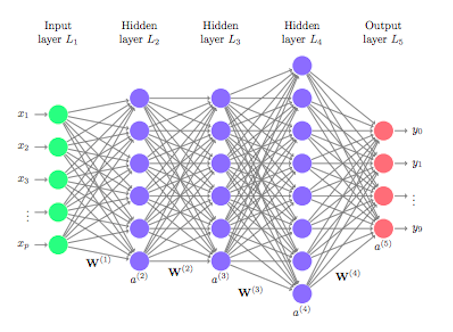
\includegraphics[scale=0.4]{deep_learning.png}
		\caption{Deep learning structure}
		\label{fig:fig0}
	\end{figure}
	\item It's even better if you put a caption on it. Figure~\ref{fig:fig0} shows a deep learning structure.
\end{itemize}
\end{frame}

\section{Make tables}
\begin{frame}{Make tables}
\begin{itemize}
	\item You can draw a table easily by referring to the following address. (https://www.tablesgenerator.com/)
\end{itemize}
\begin{table}[h]
	\centering
	\caption{Averages and standard errors (in parentheses) of RMSE and MAE values (all values multiplied by $10^3$) based on 100 samples for SVQR and QSS}
	\resizebox{\linewidth}{!}{
		\begin{tabular}{@{}crrrrr@{}}
			\toprule
			& \multicolumn{2}{c}{Case 1} &  & \multicolumn{2}{c}{Case 2} \\ \cmidrule(lr){2-3} \cmidrule(l){5-6} 
			Indices&\multicolumn{1}{c}{SVQR}&\multicolumn{1}{c}{QSS}&  &\multicolumn{1}{c}{SVQR}&\multicolumn{1}{c}{QSS}\\ \midrule\midrule
			$\tau = 0.1$&     &    &  &     &    \\
			RMSE&249.3 (1.13)&299.3 (1.34)&  &231.6 (1.30)&310.1 (0.93)    \\
			MAE&157 (0.88)&170.8 (0.93)&  &128.6 (0.71)&155.7 (0.72)    \\
			$\tau = 0.5$&    &    &  &     &    \\ \bottomrule
		\end{tabular}
	}
\end{table}
\end{frame}

\begin{frame}{Make equations}
\begin{itemize}
\item Assume $\sum(X_{i,n} - \bar{X})/(\sum (X_{i,n}-\bar{X})^2) := w_{i,n}$ and $Z_{i,n} \overset{ind}{\sim} N(0, \sigma_i^2)$.
\item Then by Lindeberg's condition,
\begin{align}
\frac{1}{\sum_{i = 1}^n \sigma_i^2}
\sum_{i = 1}^nE&\left[ w_{i,n}^2Z_{i,n}^2 I\left(\left| w_{i,n}Z_{i,n} \right| > \epsilon \sqrt{\sum_{i = 1}^n \sigma_i^2} \right) \right] \\
&\le \frac{1}{\sum_{i = 1}^n \sigma_i^2} \max_{1 \le i \le n}w_{i,n}^2 \max_{1 \le i \le n}E(Z_{i,n}^2) \rightarrow 0
\end{align}
\item Also $E(\hat{\beta}_x) = \beta_x$ and $V(Y_{i,n}) = \sigma^2$.
\item Thus, the least square slope estimator($\hat{\beta}_x$) is asymptotically normal. \\
\item And (iii), (iv) do not converge asymptotically normal by below.
\end{itemize}
\end{frame}

\section{Referencing article}
\begin{frame}{Referencing article}
  \begin{itemize}
    \item First visit google scholar cite(https://scholar.google.com/)
    \item Then click the "" icon.
    \begin{figure}[h]
    	\centering
    	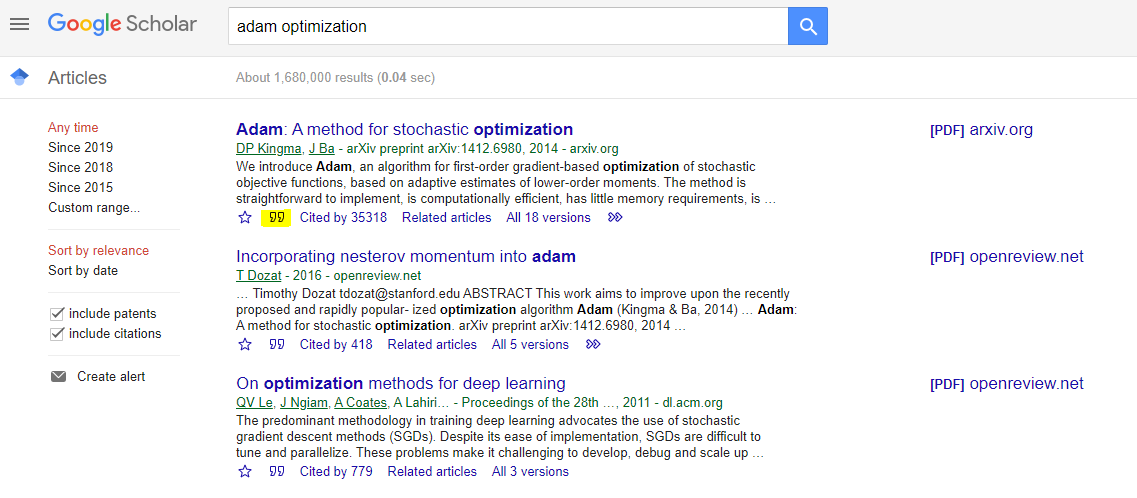
\includegraphics[scale=0.3]{google_scholar.png}
    	\caption{Google scholar page 1.}
    	\label{fig:fig1}
    \end{figure}
 \end{itemize}
\end{frame}
\begin{frame}{Referencing article}
\begin{itemize}
	\item Click the Bibtex file
	\begin{figure}[h]
		\centering
		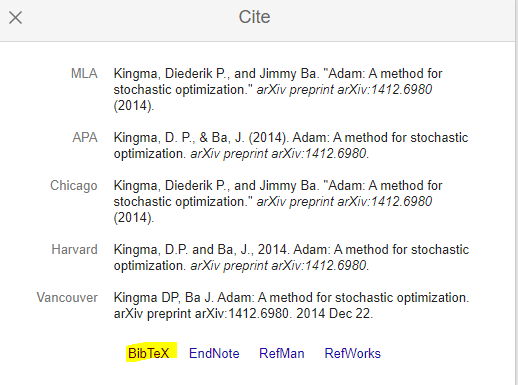
\includegraphics[scale=0.4]{google_scholar2.png}
		\caption{Google scholar page 2.}
		\label{fig:fig2}
	\end{figure}
\end{itemize}
\end{frame}
\begin{frame}{Referencing article}
\begin{itemize}
	\item Next, scrape the lines
	\begin{figure}[h]
		\centering
		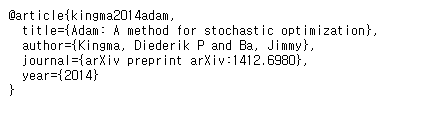
\includegraphics[scale=0.4]{google_scholar3.png}
		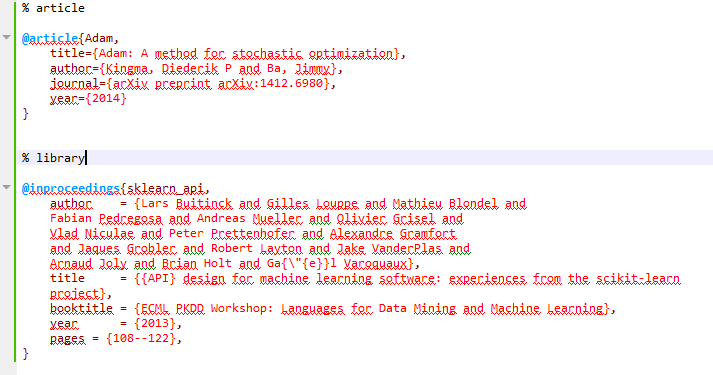
\includegraphics[scale=0.3]{google_scholar4.png}
		\caption{Google scholar page 3.}
		\label{fig:fig3}
	\end{figure}
	\item And make .bib file to your references.
	\item Notice that your .bib file \textcolor{red}{must be} with the .tex file you want to compile.
\end{itemize}
\end{frame}
\begin{frame}{Referencing article}
\begin{itemize}
	\item It is able to solve massive data set problems for using many hidden units in a layer, multiple hidden layers, weight sharing, a variety of colorful forms, and innovative learning algorithms such as Adam(\cite{Adam}).
\end{itemize}
\end{frame}

\section{Reference}
\begin{frame}{Reference}
\bibliography{references}
\end{frame}


\end{document}
